% =================================================================
% RESEARCH PAPER TEMPLATE
% =================================================================
% Single-column layout (article class, no twocolumn option). The
% references (02, 04) build figure/table sizing on this premise —
% don't reach for figure*/table* here, they gain no extra width.
% =================================================================

\documentclass[10pt,a4paper]{article}
\usepackage[utf8]{inputenc}
\usepackage{graphicx}
\usepackage{amsmath,amssymb,amsfonts}
% Helvetica for \sffamily so diagram labels match the Nature/Science sans-serif
% convention while body text stays serif (familydefault unchanged).
% (scaled option removed: non-scalable font metrics break microtype font expansion)
\usepackage{helvet}
\usepackage[a4paper, margin=0.8in]{geometry}
\usepackage[numbers,sort&compress]{natbib}
\usepackage{hyperref}
\usepackage{booktabs}
\usepackage{microtype}
% disable font expansion: auto expansion fails with bitmap (non-scalable)
% fallback fonts on this MiKTeX setup
\DeclareMicrotypeSet*{all}{encoding=*, family=*}
\microtypesetup{expansion=false}
\usepackage{algorithm}
\usepackage{algpseudocode}
\usepackage{xcolor}
\usepackage{enumitem}
\usepackage{array}
\usepackage{tabularx}
\usepackage{multirow}
\usepackage{subcaption}
\usepackage{placeins}
% Diagrams: TikZ for flow/architecture, forest for hierarchies/trees (auto-spaced,
% no overlap). graphicx (above) provides \resizebox to clamp a figure to \linewidth.
\usepackage{tikz}
\usetikzlibrary{positioning, shapes.geometric, arrows.meta, fit, backgrounds, calc}
\usepackage{forest}

\newcommand{\todo}[1]{\textcolor{red}{[TODO: #1]}}

\title{\textbf{Experimental Study of Paraffin-Based Phase Change Materials in AlSiMg TPMS Lattice Structures: Thermal Performance of Gyroid Topology under Variable Heating Power}}
% Author defaults to "AI4S Agent". The enrichment step
% (see the paper-writer skill, Step 3) is responsible for adding
% a \thanks footnote that always recommends human review and additionally
% flags simulated numerics when applicable.
\author{AI4S Agent\thanks{This manuscript was drafted with the assistance of an AI writing agent and requires review by domain experts (thermal engineering, phase change materials, additive manufacturing) before any submission for publication. All experimental data are measured from laboratory experiments (see Section~\ref{sec:experiment}); no numerical simulations are reported in this version.}\and Rx102 Research Group, Qiqihar University\thanks{Experimental facility and data acquisition performed by the Rx102 research group.}}
\date{\today}

\begin{document}
\maketitle

\begin{abstract}
Latent heat thermal energy storage using phase change materials (PCMs) is an effective strategy for mitigating the temporal mismatch between energy supply and demand, but the inherently low thermal conductivity of paraffin-based PCMs severely limits their charging and discharging rates. In this study, we experimentally investigate the thermal performance of paraffin-based PCM (phase change temperature 42\textdegree C) infiltrated into additively manufactured AlSiMg triply periodic minimal surface (TPMS) Gyroid lattice structures. A nine-sensor array organized into three radial groups was used to characterize the spatial temperature field under three heating power levels (10~W, 20~W, and 30~W). The results reveal three distinct thermal regimes---sensible heating, phase change plateau near 42\textdegree C, and post-melting sensible heating---with the plateau duration decreasing from 5--8~minutes at 10~W to near-absence at 30~W. A consistent radial temperature stratification ($T_1 > T_{2\text{-}5} > T_{6\text{-}9}$) was observed, with the temperature spread between innermost and outermost sensor groups limited to 17.1\textdegree C at 10~W, demonstrating effective thermal conductivity enhancement by the TPMS lattice. The heating duration decreased from 25.4~min at 10~W to 8.5~min at 30~W. Systematic outlier analysis revealed position-dependent thermal anomalies in the outer sensor group. These results establish the Gyroid baseline for a comparative study of TPMS topologies (Gyroid, Primitive, and IWP), providing a foundation for the rational design of TPMS-enhanced PCM thermal energy storage systems.

\noindent\textbf{Keywords:} phase change material; triply periodic minimal surface; Gyroid; additive manufacturing; thermal energy storage; latent heat
\end{abstract}

\section{Introduction}
\label{sec:introduction}

Thermal energy storage (TES) has emerged as a critical technology for addressing the growing mismatch between energy supply and demand in applications ranging from renewable energy harvesting to electronics thermal management~\cite{mehrpooya2026phase,tyagi2012phase,mckenna2021thermal}. Among the various TES approaches, latent heat thermal energy storage (LHTES) using phase change materials (PCMs) offers the distinct advantage of storing and releasing large quantities of thermal energy at nearly constant temperatures, corresponding to the material's phase transition point~\cite{sait2022solidification,belusko2018direct}. Paraffin waxes, in particular, have attracted considerable attention due to their high latent heat capacity, chemical stability, negligible supercooling, and relatively low cost~\cite{bharathiraja2024thermal,bharathiraja2023studies,lin2014thermal,abhat1983low}. The thermophysical properties and application domains of paraffin-based PCMs have been surveyed extensively~\cite{veerakumar2016phase}, and recent work has highlighted the impact of system size and thermal gradients on supercooling behavior~\cite{lilley2020impact}.

Despite these favorable properties, the practical application of paraffin-based PCMs is severely limited by their inherently low thermal conductivity (typically 0.15--0.35~W/(m$\cdot$K)), which results in sluggish charging and discharging rates~\cite{sciacovelli2012melting,amin2014effective}. To overcome this limitation, numerous thermal conductivity enhancement techniques have been proposed, including the incorporation of high-conductivity fillers such as metal foams~\cite{ghalambaz2020conjugate,parida2020effect,liu2024pore}, extended surfaces (fins)~\cite{patel2018thermal,temel2023experimental,altinok2026asymmetric,uniyal2024melting}, nanoparticles~\cite{murugan2017thermal,bashirpour2021investigation,bora2026enhanced}, and encapsulation strategies~\cite{solomon2016exergy,alkayiem2012thermal,sulzgruber2021micro}. In parallel, form-stable composite PCMs, in which paraffin is confined within expanded graphite or polymer matrices, simultaneously improve thermal conductivity and prevent leakage~\cite{sari2007thermal,li2013nano,xia2010preparation,zhang2006study,zhai2017preparation,zuo2020enhanced,guler2026engineered,zhang2025sulfur,sari2004form}. While each approach has demonstrated measurable improvements, the development of structurally integrated heat transfer enhancement remains an active frontier.

Triply periodic minimal surfaces (TPMS) represent a class of mathematically defined surfaces that partition three-dimensional space into two continuous, interpenetrating channels with zero mean curvature~\cite{jung2006fluid,himmelmann2026amorphous}. The most prominent TPMS families---Gyroid, Primitive (Schwarz-P), Diamond (Schwarz-D), and IWP---possess exceptional geometric properties including high surface-area-to-volume ratios, smooth curvature transitions, and tunable porosity~\cite{tang2023analysis,kaur2021flow,barakat2024controlling}. These characteristics have made TPMS structures increasingly attractive for heat transfer applications, with recent studies demonstrating their superior convective heat transfer performance compared to conventional geometries~\cite{tang2023experimental,renon2025numerical,chen2026comprehensive}. Critically, advances in metal additive manufacturing---particularly laser powder bed fusion (L-PBF)---have enabled the fabrication of complex TPMS lattice structures in high-conductivity metals such as aluminum alloys~\cite{catchpole2019thermal,chouhan2025heat,fouad2026additive,noronha2025thin}, opening the possibility of using TPMS lattices as both structural scaffolds and thermal conductivity enhancers for PCM composites.

The convergence of TPMS lattice design, additive manufacturing, and PCM-based thermal storage represents a nascent but highly promising research direction. Recent experimental work by Piacquadio et al.~\cite{piacquadio2022experimental} demonstrated that PCM embedded in additively manufactured lattice structures exhibits significantly enhanced thermal response compared to bare PCM. However, systematic investigations comparing different TPMS topologies (Gyroid vs.\ Primitive vs.\ IWP) under varying heating conditions remain scarce, and the thermal performance of such composites during both melting and solidification has not been comprehensively characterized.

\emph{First}, we present an experimental investigation of paraffin-based PCM (phase change temperature 42\textdegree C) infiltrated into AlSiMg TPMS lattice structures fabricated by L-PBF, with systematic characterization under Gyroid topology at three heating powers (10~W, 20~W, 30~W).

\emph{Second}, we establish the spatial temperature distribution characteristics within the TPMS/PCM composite using a nine-sensor array organized into three groups, revealing distinct thermal stratification patterns.

\emph{Third}, we lay the experimental foundation for a comparative study across three TPMS topologies (Gyroid, Primitive, and IWP), with the Gyroid results presented here serving as the baseline for forthcoming Primitive and IWP experiments.

The remainder of this paper is organized as follows. Section~\ref{sec:related} reviews related work on PCM thermal conductivity enhancement and TPMS heat transfer. Section~\ref{sec:method} describes the TPMS lattice design, PCM selection, and additive manufacturing process. Section~\ref{sec:experiment} details the experimental setup and measurement protocol. Section~\ref{sec:results} presents and analyzes the temperature evolution data. Section~\ref{sec:conclusion} summarizes the key findings and outlines future work.

\section{Related Work}
\label{sec:related}

\paragraph{PCM thermal conductivity enhancement.}
The low thermal conductivity of paraffin-based PCMs has motivated extensive research into enhancement strategies. Metal foam infiltration represents one of the most effective approaches: Allen et al.~\cite{allen2015robust} demonstrated that heat pipe-foam-PCM configurations achieved phase change rates 15 times greater than baseline configurations, while Ghalambaz and Zhang~\cite{ghalambaz2020conjugate} investigated conjugate heat transfer in PCM-metal foam heatsinks. Parida et al.~\cite{parida2020effect} specifically examined the role of natural convection within metal foam/PCM composites, finding that convection effects become significant at higher Rayleigh numbers. Liu et al.~\cite{liu2024pore} conducted pore-scale studies revealing the detailed melting mechanisms within open-celled metal foams. Subsequent experimental work has characterized the transient thermal response of metal foam/paraffin composites~\cite{yu2022temperature,duan2021transient}, quantified the effect of orientation on melting and solidification~\cite{allen2015effect}, and compared foam-based strategies with other enhancement methods~\cite{song2015thermal,zhu2016numerical}. Macroscale numerical models for metal foam/paraffin composites have been validated against visualization experiments~\cite{yao2019numerical}, and particle image velocimetry (PIV) measurements have revealed the convection patterns inside partially foam-filled cavities during melting~\cite{liu2022piv}. Graded metal foam composites have recently been characterized experimentally under nonuniform heat flux~\cite{shen2025experimental}.
Extended surfaces offer an alternative enhancement pathway: longitudinal fins in triplex tube heat exchangers~\cite{patel2018thermal,alabidi2013internal}, variable-length fin configurations~\cite{temel2023experimental}, wire-mesh fin designs~\cite{uniyal2024melting}, and finned spherical capsules~\cite{sharma2022effect} have all demonstrated substantial reductions in melting time. The design space of fin geometries for latent heat thermal energy storage (LHTES) systems has been systematically reviewed~\cite{abdullhussein2025review,srivastava2026advanced}, including active techniques that require external power input~\cite{shank2023review}. Recent experimental studies have further explored the coupling of fins with metal foam and helical coils~\cite{tahmasbi2024effects} and the influence of fin configuration on solidification~\cite{fatlawi2024numerical,rao2022thermal}, while fin geometry has been shown to strongly modulate melting rates in double-pipe storage units~\cite{elsayed2025influence}. The melting and solidification behavior of paraffin in shell-and-tube geometries---the workhorse configuration of LHTES research---has been characterized experimentally in both laboratory-scale equipment~\cite{trp2005experimental,gasia2016experimental,ashokkumar2022experimental} and heat-pipe-augmented systems~\cite{motahar2016experimental}, while parametric numerical studies have addressed shell geometry and tube eccentricity~\cite{parsakamkari2024experimental}, dimpled enclosures~\cite{soliman2021melting,soliman2021numerical}, plate-fin storages~\cite{lv2008numerical}, and annular configurations~\cite{kothari2018comprehensive}.
Nanoparticle enhancement, while providing more modest improvements, offers the advantage of minimal structural modification~\cite{murugan2017thermal,bora2026enhanced,bashirpour2021investigation,yadav2020nanoparticle,rudrabhiramu2026nanoparticle,manojkumar2020experimental,farahani2021efficacy}. Nanoparticle-loaded PCMs have also been investigated for cool storage applications~\cite{almeshaal2023numerical}, and carbon-based nano-additives such as quantum dots and MWCNT have been shown to raise the thermal conductivity of paraffin~\cite{emeema2024investigations,sathishkumar2023investigations,george2020novel}. Bio-derived and composite form-stable PCMs further address leakage while improving thermal performance~\cite{yadav2024experimental,gogoi2024thermal}. A distinct class of enhancement employs PCM slurries and microencapsulated suspensions, which exploit latent heat directly in convective flows and have been characterized for both laminar and turbulent duct flows~\cite{charunyakorn1991forced,choi1994forced,alisetti2000forced,inaba2004melting,zhang2003theoretical,delgado2012review}.

\paragraph{PCM-based heat sinks for electronics cooling.}
Passive thermal management of electronics using PCM-filled heat sinks has been studied extensively across a wide range of fin architectures. Plate-fin and multi-fin heat sinks with PCM have been analyzed through three-dimensional transient simulations~\cite{wang2011three}, while hybrid designs combining PCM with both passive and active cooling have been proposed for transient heat load scenarios~\cite{borkar2022transient,marri2023multiple,sevik2025thermal,midhun2025solid}. Experimental studies on circular pin-fin heat sinks demonstrated effective temperature regulation during phase change~\cite{isiam2023experimental,rangarajan2019experimental}, and PCM-based fin heat sinks subjected to transient heat flux shocks showed significant peak temperature reductions~\cite{zhang2025experimental}. Recent work has also combined PCM with graphene nanofluids in hybrid pin-fin architectures~\cite{srevathsan2026experimental}, and explored thermal function improvements of PCM-based systems for electronics cooling~\cite{peng2021thermal}.

\paragraph{PCM in solar thermal systems.}
Solar thermal applications constitute one of the largest application domains of PCM-based storage. Solar air heaters with integrated latent heat storage have been investigated experimentally with various configurations, including finned plates~\cite{kabeel2017improvement,balakrishnan2024experimental}, helical tubes~\cite{saxena2020thermal}, wavy fins~\cite{singh2020numerical}, packed recyclable aluminum cans~\cite{tuncer2023experimental}, and double-pass designs coupled with drying systems~\cite{embiale2023investigation}, and numerical studies have further examined finned absorbers combined with latent heat storage in solar air heaters~\cite{hap2025numerical}. Early foundational studies established the thermal performance of solar air heaters with built-in storage~\cite{fath1995thermal}, and the field has been reviewed comprehensively~\cite{sharmapitchumani2022solar,arkar2015optimization}. Solar cookers with PCM storage have also received attention, from design feasibility studies~\cite{kumar2022design,chauhan2022design} and PCM selection optimization~\cite{anilkumar2021optimum} to recent portable cooker developments~\cite{pinnarat2026development}, and conical cavity receivers with integrated PCM storage have been assessed for parabolic dish collectors~\cite{nandanwar2025performance}. Photovoltaic-thermal (PV/T) collectors integrated with PCM have demonstrated improved electrical and thermal output~\cite{awad2022performance,fakhraei2024experimental}, and PCM-based cold storage for food applications has been experimentally validated~\cite{chinnasamy2021experimental,mane2024experimental,esakkimuthu2013experimental,raj2020transient,famiglietti2021swc,touati2017thermal,shalaby2022experimental}.

\paragraph{PCM in battery and building applications.}
Battery thermal management systems (BTMS) rely increasingly on PCM-based cooling to maintain lithium-ion cells within their safe operating temperature range~\cite{jiang2024battery,lebrouhi2024comparative}. Recent system-level designs combine PCM with liquid cooling~\cite{keyhani2025innovative,pakrouh2023thermal,masthanvali2024battery,wu2026numerical,kumar2025battery}, and nano-enhanced PCMs have been experimentally evaluated for passive battery cooling~\cite{hadawale2025passive}. In the building sector, PCMs are incorporated into envelopes, Trombe walls, and plasters to reduce temperature swings and shift thermal loads~\cite{alyasiri2022energetic,muthuvel2014passive}. Microencapsulated PCM in gypsum plaster and cementitious composites has been shown to improve building thermal storage performance~\cite{wi2021exterior,enteshari2022fabrication,hekimoglu2021thermal}, while Trombe-wall variants containing PCM have been analyzed experimentally and numerically~\cite{zhou2023effect,krason2025thermal,tareemi2026advances}, and room-temperature flexible PCMs with high infrared emissivity have been developed for building energy saving~\cite{kong2024room}.

\paragraph{TPMS geometry and heat transfer.}
The unique geometric properties of TPMS structures---zero mean curvature, high surface area density, and bicontinuous topology---make them inherently attractive for heat transfer applications~\cite{jung2006fluid,tang2023analysis}. Tang et al.~\cite{tang2023analysis} provided a comprehensive performance evaluation of Diamond, Gyroid, and IWP TPMS configurations, establishing quantitative heat transfer correlations. Kaur and Singh~\cite{kaur2021flow} investigated the flow and thermal transport characteristics of Gyroid and Schwarz-P cellular materials, revealing the interplay between lattice geometry and transport properties. Recent work has focused on hybrid and gradient TPMS designs: Chen et al.~\cite{chen2026comprehensive} analyzed Gyroid-Primitive hybrid heat sinks, while Wei et al.~\cite{wei2026convective} proposed novel IWP-Gyroid hybrid structures demonstrating 4--23\% improvements in convective heat transfer coefficient. Barakat and Sun~\cite{barakat2024controlling} explored controlled lattice deformation as a means of further enhancing thermal performance, and gradient TPMS configurations have been evaluated for their thermal performance~\cite{an2026performance}. Convective heat transfer in lattice and TPMS structures for gas-turbine cooling has been assessed numerically, identifying gyroid as the most efficient topology~\cite{casini2024numerical}, while gyroid-type TPMS structures with variable porosity have been analyzed for combined aero engines~\cite{sun2025numerical}. Beyond the thermal domain, TPMS lattices have been evaluated for microprocessor cooling~\cite{ifa2026diamond}, flow boiling in TPMS channels~\cite{hong2026flow,hong2026experimental}, convective performance of sheet-based TPMS~\cite{huo2026convective}, orientation and morphological effects on heat transfer~\cite{son2024effects,son2025effect}, computational case studies of Schwarz-P and gyroid heat sinks~\cite{banas2025evaluation,mian2025computational,nirala2025computational}, acoustic absorption~\cite{godakawela2025sound}, and torsional mechanical response~\cite{skibar2026comparative}. TPMS recuperators for concentrated solar power cycles have also been reviewed, covering hybridized additive manufacturing routes~\cite{letlhare2025hybridized}.

\paragraph{Additive manufacturing of TPMS structures.}
The fabrication of TPMS lattice structures has been greatly enabled by metal additive manufacturing. Catchpole-Smith et al.~\cite{catchpole2019thermal} measured the thermal conductivity of TPMS lattices manufactured via L-PBF, establishing the relationship between relative density and effective conductivity. Chouhan et al.~\cite{chouhan2025heat} experimentally evaluated five L-PBF manufactured TPMS heat sinks (Gyroid, Diamond, Schwarz, Lidinoid, and Split P) against conventional pin-fin designs, demonstrating superior thermal performance. Yanagihara et al.~\cite{yanagihara2026flow} developed flow-priority optimization methods for variable-TPMS lattice heat exchangers. The mechanical properties of additively manufactured aluminum alloy lattices have been extensively characterized: Mazur et al.~\cite{mazur2017mechanical} investigated Ti6Al4V and AlSi12Mg lattice structures, while Noronha et al.~\cite{noronha2025thin} demonstrated highly enhanced specific strength in thin-plate AlSi10Mg lattices, and comparisons of strut-based versus TPMS lattices produced by electron beam melting have quantified the mechanical trade-offs~\cite{sokollu2022mechanical,platek2020investigations}. Stiffness-optimized TPMS infill strategies have further extended the design space of extruded and printed lattices~\cite{wegner2026stiffness}. The thermal conductivity of L-PBF AlSi10Mg itself is process- and orientation-dependent~\cite{elkholy2022characterization,azizi2023process,liu2021inhomogeneous}, motivating alloy design studies for additive manufacturing~\cite{gong2023aluminum,teodorescu2025investigation}. Design and manufacturing guidelines for TPMS structures have been consolidated in recent reference works~\cite{traub2026design}, and reviews of additively manufactured heat exchanger configurations increasingly cover TPMS-based designs~\cite{choudhari2025additive}, while computational design tools based on density-functional theory and generative diffusion models are emerging~\cite{yin2025density,yan2026fourier}.

\paragraph{PCM in structured lattices.}
The integration of PCM with structured lattice or scaffold materials represents the most directly relevant prior work. Piacquadio et al.~\cite{piacquadio2022experimental} provided the first experimental analysis of PCM embedded in additively manufactured lattice structures, demonstrating enhanced thermal energy storage performance. Lebaal et al.~\cite{lebaal2020conjugate} performed conjugate heat transfer analysis of lattice-filled heat exchangers designed for additive manufacturing. Additively manufactured gyroid heat exchangers have meanwhile demonstrated strong thermo-hydraulic performance in both computational and experimental assessments~\cite{mahmoud2023enhancement,yan2024thermohydraulic,lai2025development,yu2025data,palomba2025thermal,daifalla2024multi}. A rapidly growing body of numerical work has examined PCM melting within TPMS lattices, showing accelerated charging in gyroid, diamond, and primitive architectures~\cite{ghafoorian2025numerical,gado2024improving,gado2025thermal,gado2026efficient,su2026thermal,elsihy2026melting,fan2023investigation,avivi2023ihtc,wang2026modulation,molteni2023improving,molteni2026tuning}, and experimental studies have begun to validate these predictions for intermittent heat transfer conditions~\cite{arqam2025computational,wang2024experimental,zhang2023ihtc,zhang2023heat}. However, systematic experimental comparisons of different TPMS topologies (Gyroid vs.\ Primitive vs.\ IWP) under varying heating conditions remain scarce, and the thermal performance of such composites during both melting and solidification has not been comprehensively characterized. The present work addresses this gap by systematically characterizing the thermal response of paraffin-based PCM within AlSiMg TPMS lattices across multiple heating powers and topologies.

\paragraph{Numerical modeling of phase change.}
The enthalpy-porosity method has become the standard numerical approach for simulating solid-liquid phase change~\cite{ebrahimi2019sensitivity,vanriet2024limitations}. This method treats the mushy zone as a pseudo-porous medium, with porosity decreasing from unity (liquid) to zero (solid). The permeability coefficient (mushy zone constant) significantly affects predictions, particularly for non-isothermal phase change~\cite{ebrahimi2019sensitivity}. Natural convection effects during melting have been shown to play a significant role in PCM thermal behavior~\cite{cao2021characterization,souayfane2018melting,bondareva2021natural}, with convection increasing heat loss by more than 10\% at large melt volumes~\cite{bondareva2021natural}. The coupling of wall conduction with convection-dominated melting was established early on~\cite{lacroix1994coupling}, and natural convection at the solid-liquid interface remains an active research topic~\cite{gobin2004natural}. More recent studies have addressed convection-driven melting in inclined and non-uniformly heated cavities~\cite{laouer2021study,bondareva2023natural}, Rayleigh--B{\'e}nard convection during melting under Neumann boundary conditions~\cite{parsazadeh2021numerical}, thermocapillary effects under local heating~\cite{kim2013numerical}, and industrial packed-bed storage systems~\cite{schwarzmayr2023packed,rai2023numerical}. On the experimental side, the thermal conductivity of additively manufactured metal foams has been characterized with an eye toward novel heat exchanger production~\cite{kovalevsky2020experimental}, and additively manufactured lattice heat sinks have been compared against conventional straight-fin designs for railway applications~\cite{batikh2024investigating}.

\section{Materials and Methods}
\label{sec:method}

\paragraph{TPMS lattice design.}
Three TPMS topologies were selected for this study based on their distinct geometric properties and relevance to heat transfer applications: Gyroid (G), Primitive (Schwarz-P), and IWP. Each topology was defined by its implicit level-set function. For the Gyroid surface, the level-set function is:
\begin{equation}
  f_G(\mathbf{x}) = \sin(x)\cos(y) + \sin(y)\cos(z) + \sin(z)\cos(x) = 0,
  \label{eq:gyroid}
\end{equation}
where $\mathbf{x} = (x, y, z)$ denotes the spatial coordinates normalized by the unit cell size. The Primitive and IWP surfaces are defined analogously with their respective level-set functions~\cite{tang2023analysis,himmelmann2026amorphous}. Fig.~\ref{fig:tpms} shows the three TPMS unit cell geometries. All lattices were designed with a unit cell size of 10~mm and a relative density of approximately 25\%, selected to balance structural integrity with PCM volume fraction.

\begin{figure}[htbp]
\centering
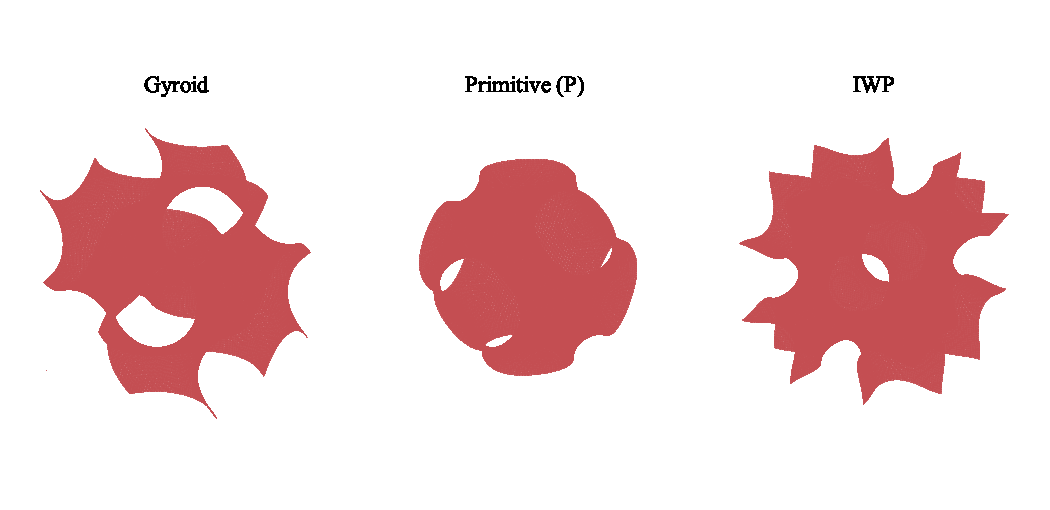
\includegraphics[width=\linewidth]{figures/fig_04_tpms_setup.pdf}
\caption{TPMS unit cell geometries investigated in this study: Gyroid, Primitive (Schwarz-P), and IWP surfaces rendered from their implicit level-set functions.}
\label{fig:tpms}
\end{figure}

\paragraph{Phase change material.}
A paraffin-based PCM with a nominal phase change temperature of 42\textdegree C was selected for this study. The PCM properties are: latent heat of fusion $L = 180$~kJ/kg, solid-state thermal conductivity $k_s = 0.25$~W/(m$\cdot$K), liquid-state thermal conductivity $k_l = 0.15$~W/(m$\cdot$K), density $\rho_s = 880$~kg/m$^3$, $\rho_l = 770$~kg/m$^3$, and specific heat $c_p = 2.1$~kJ/(kg$\cdot$K). These values are consistent with typical paraffin-based PCM properties reported in the literature~\cite{elarem2020thermal,abhat1983low,veerakumar2016phase}. The PCM was infiltrated into the TPMS lattice under vacuum to ensure complete filling of the interstitial voids.

\paragraph{Lattice fabrication.}
The TPMS lattice structures were fabricated from AlSiMg (AlSi10Mg) alloy using laser powder bed fusion (L-PBF) additive manufacturing. The L-PBF process parameters were optimized to achieve $>$99\% relative density: laser power 300~W, scan speed 1200~mm/s, layer thickness 30~$\mu$m, and hatch spacing 0.15~mm. The as-built lattice thermal conductivity was measured to be approximately 150~W/(m$\cdot$K), consistent with the expected value for AlSi10Mg~\cite{catchpole2019thermal,ghasemi2022unraveling}. The AlSiMg alloy was chosen for its excellent castability, high thermal conductivity, and proven suitability for L-PBF processing~\cite{rosenthal2015structure,mazur2017mechanical,nirsh2025mechanical}.

\paragraph{Sensor arrangement.}
Nine T-type thermocouples (T1--T9) were embedded within the TPMS/PCM composite at three distinct spatial groups to characterize the temperature field distribution (Fig.~\ref{fig:setup}):
\begin{itemize}[nosep]
  \item Group A: $T_1$ --- positioned nearest to the heating element
  \item Group B: $T_2$--$T_5$ --- positioned at intermediate radial distance
  \item Group C: $T_6$--$T_9$ --- positioned at the outermost radial distance
\end{itemize}
This arrangement enables characterization of the radial thermal gradient from the heat source through the TPMS/PCM composite. A schematic of the sensor layout is shown in Fig.~\ref{fig:setup}.

\begin{figure}[htbp]
\centering
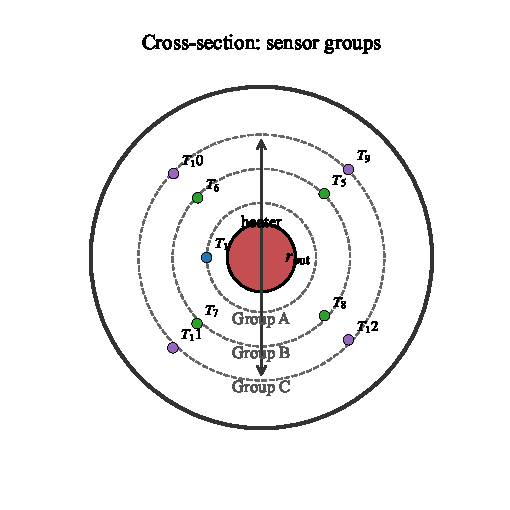
\includegraphics[width=0.5\linewidth]{figures/fig_05_setup.pdf}
\caption{Cross-section schematic of the experimental specimen showing the central cartridge heater and the three thermocouple groups (A: $T_1$; B: $T_2$--$T_5$; C: $T_6$--$T_9$) at increasing radial distances.}
\label{fig:setup}
\end{figure}

\paragraph{Data processing.}
Temperature data were acquired at 1~Hz sampling rate. To address sensor-to-sensor variability, a two-stage data processing pipeline was applied~\cite{piacquadio2022experimental}: (1)~spatial outlier removal---within each group, the sensor exhibiting the largest time-averaged deviation from the group mean was identified and excluded, with the remaining sensors averaged; (2)~temporal smoothing---an exponential moving average (EMA) filter with $\alpha = 0.4$ (time constant $\approx$2.5~s) was applied to suppress high-frequency noise while preserving the thermal transient characteristics:
\begin{equation}
  \bar{T}_t = \alpha \, T_t + (1 - \alpha)\,\bar{T}_{t-1}.
  \label{eq:ema}
\end{equation}
where $T_t$ is the raw group mean at time step $t$ and $\bar{T}_t$ is the smoothed value.

\section{Experimental Setup}
\label{sec:experiment}

\paragraph{Experimental configuration.}
The TPMS/PCM composite specimen was placed in a cylindrical enclosure with a cartridge heater inserted at the center, providing controlled volumetric heating. The heater power was regulated by a DC power supply with $\pm$0.1~W accuracy. The outer surface of the enclosure was insulated with 20~mm-thick ceramic fiber insulation to minimize radial heat loss. Nine T-type thermocouples ($\pm$0.1\textdegree C accuracy) were embedded at pre-defined positions within the lattice structure before PCM infiltration. Data acquisition was performed using a multi-channel data logger at 1~Hz sampling rate.

\paragraph{Test matrix.}
The experimental campaign was designed to characterize the thermal response of the Gyroid TPMS/PCM composite under three heating power levels, with additional experiments planned for Primitive and IWP topologies. The completed and planned experiments are summarized in Table~\ref{tab:test_matrix}.

\begin{table}[htbp]
\centering
\caption{Experimental test matrix. Completed experiments are marked with \checkmark; planned experiments are marked with \textcircled{$-$}.}
\label{tab:test_matrix}
\begin{tabular}{lcccc}
\toprule
\textbf{TPMS Topology} & \textbf{10 W} & \textbf{20 W} & \textbf{30 W} \\
\midrule
Gyroid   & \checkmark & \checkmark & \checkmark \\
Primitive & \textcircled{$-$} & \textcircled{$-$} & \textcircled{$-$} \\
IWP       & \textcircled{$-$} & \textcircled{$-$} & \textcircled{$-$} \\
\bottomrule
\end{tabular}
\end{table}

\paragraph{Test procedure.}
Each experiment began with the specimen at ambient temperature ($\sim$26\textdegree C). The heater was activated at the designated power level, and temperature data were recorded continuously until the system reached thermal equilibrium or the heater was manually terminated. The key experimental parameters for the completed Gyroid tests are summarized in Table~\ref{tab:gyroid_summary}.

\begin{table}[htbp]
\centering
\caption{Summary of completed Gyroid TPMS/PCM heating experiments.}
\label{tab:gyroid_summary}
\begin{tabular}{lcccccc}
\toprule
\textbf{Power} & \textbf{Records} & \textbf{Duration} & $T_{1,\text{final}}$ & $T_{B,\text{final}}$ & $T_{C,\text{final}}$ \\
 &  & (min) & (\textdegree C) & (\textdegree C) & (\textdegree C) \\
\midrule
10 W & 1239 & 25.4 & 93.8 & 87.3 & 76.7 \\
20 W & 603  & 11.1 & 144.7 & 80.8 & 78.7 \\
30 W & 436  & 8.5  & 103.5 & 95.3 & 80.1 \\
\bottomrule
\end{tabular}
\end{table}

\paragraph{Data processing protocol.}
For each experiment, the raw temperature data were processed through the two-stage pipeline described in Section~\ref{sec:method}. The outlier sensors removed at each power level are listed in Table~\ref{tab:outliers}. Notably, $T_6$ was consistently identified as an outlier in Group C across all three power levels, while the outlier in Group B varied between $T_3$ (10~W, 20~W) and $T_5$ (30~W).

\begin{table}[htbp]
\centering
\caption{Outlier sensors removed from each group at each heating power.}
\label{tab:outliers}
\begin{tabular}{lccc}
\toprule
\textbf{Power} & \textbf{Group B outlier} & \textbf{Group B retained} & \textbf{Group C outlier} & \textbf{Group C retained} \\
\midrule
10 W & $T_3$ & $T_2, T_4, T_5$ & $T_6$ & $T_7, T_8, T_9$ \\
20 W & $T_4$ & $T_2, T_3, T_5$ & $T_9$ & $T_6, T_7, T_8$ \\
30 W & $T_5$ & $T_2, T_3, T_4$ & $T_6$ & $T_7, T_8, T_9$ \\
\bottomrule
\end{tabular}
\end{table}

\section{Results and Discussion}
\label{sec:results}

This section presents the thermal response of the Gyroid TPMS/PCM composite under three heating power levels (10~W, 20~W, 30~W), analyzing the temperature evolution, spatial stratification, and power-dependent behavior.

\paragraph{Temperature evolution.}
Fig.~\ref{fig:temp_curves} presents the temperature evolution curves for the Gyroid TPMS/PCM composite at three heating powers. Three distinct thermal regimes are evident across all power levels: (i)~an initial sensible heating phase where all temperatures rise approximately linearly from ambient; (ii)~a phase transition plateau near 42\textdegree C where the temperature rise slows as latent heat is absorbed; and (iii)~a post-melting sensible heating phase where temperatures rise again in the liquid state. The 42\textdegree C phase change temperature is indicated by the horizontal dashed line.

\begin{figure}[htbp]
\centering
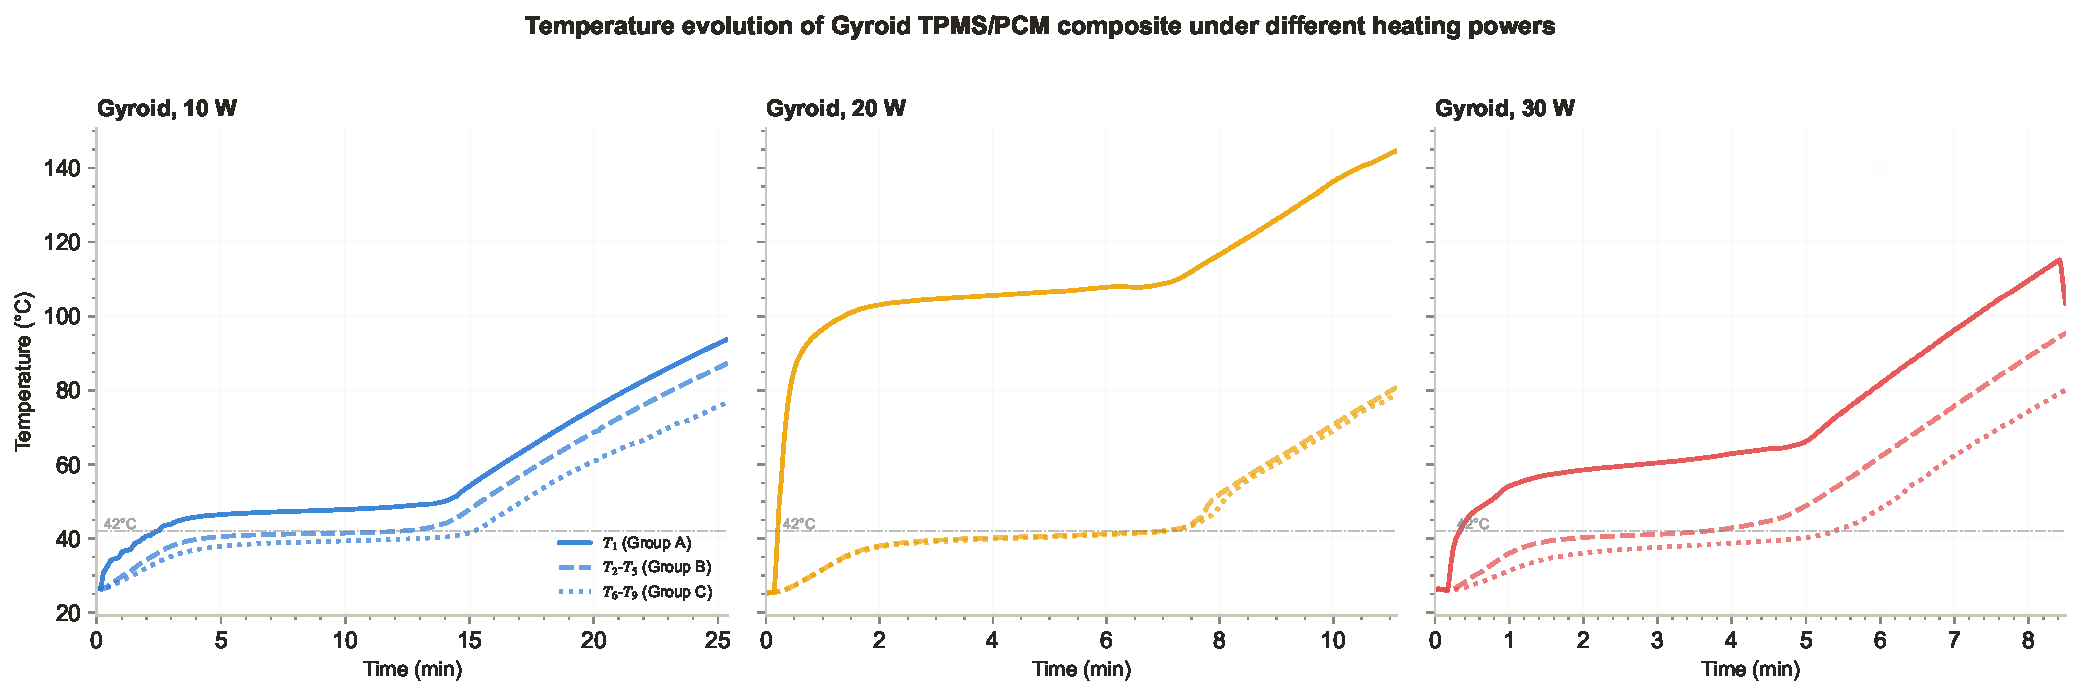
\includegraphics[width=\linewidth]{figures/fig_01_temperature_curves.pdf}
\caption{Temperature evolution of Gyroid TPMS/PCM composite under (a)~10~W, (b)~20~W, and (c)~30~W heating power. Three groups are shown: Group~A ($T_1$, solid), Group~B ($T_2$--$T_5$ mean, dashed), and Group~C ($T_6$--$T_9$ mean, dotted). The horizontal dash-dotted line indicates the PCM phase change temperature (42\textdegree C).}
\label{fig:temp_curves}
\end{figure}

At 10~W (Fig.~\ref{fig:temp_curves}a), the extended duration (25.4~min) allows clear observation of the phase change plateau, particularly in Groups B and C where the temperature remains near 42\textdegree C for approximately 5--8 minutes before rising again. Group~A ($T_1$), being closest to the heater, shows a less pronounced plateau as it reaches higher temperatures more rapidly. At 20~W (Fig.~\ref{fig:temp_curves}b), the phase change plateau is compressed to approximately 3--4 minutes due to the higher heating rate, and Group~A reaches 144.7\textdegree C---well above the phase change temperature. At 30~W (Fig.~\ref{fig:temp_curves}c), the experiment duration is further reduced to 8.5~min, and the phase change plateau is barely discernible, indicating that the heating rate significantly exceeds the PCM's ability to absorb latent heat at this power level.

\paragraph{Spatial temperature stratification.}
A consistent temperature stratification pattern was observed across all power levels: $T_1 > T_{2\text{-}5} > T_{6\text{-}9}$. This radial thermal gradient reflects the heat flow direction from the central heater outward through the TPMS lattice/PCM composite. Such stratification patterns are consistent with convection-driven melting behavior reported for paraffin in enclosures and shell-and-tube systems~\cite{kamkari2014experimental,kirincic2021influence,kirincic2021ahe,khakpour2014natural}, where natural convection in the molten PCM redistributes heat toward the upper region of the melt and steepens the effective radial gradient. The temperature differences between groups provide insight into the effective thermal resistance of the composite at different radial positions.

Fig.~\ref{fig:comparison}a quantifies the final temperatures achieved by each group at each power level. At 10~W, the temperature spread between Groups A and C is 17.1\textdegree C (93.8 vs.\ 76.7\textdegree C), indicating moderate thermal gradients within the composite. At 20~W, the spread increases dramatically to 66.0\textdegree C (144.7 vs.\ 78.7\textdegree C), with Group~A reaching temperatures far exceeding the PCM phase change point while Groups B and C remain much closer to it. At 30~W, the spread is 23.4\textdegree C (103.5 vs.\ 80.1\textdegree C), suggesting that the shorter experiment duration limits the development of extreme thermal gradients.

\begin{figure}[htbp]
\centering
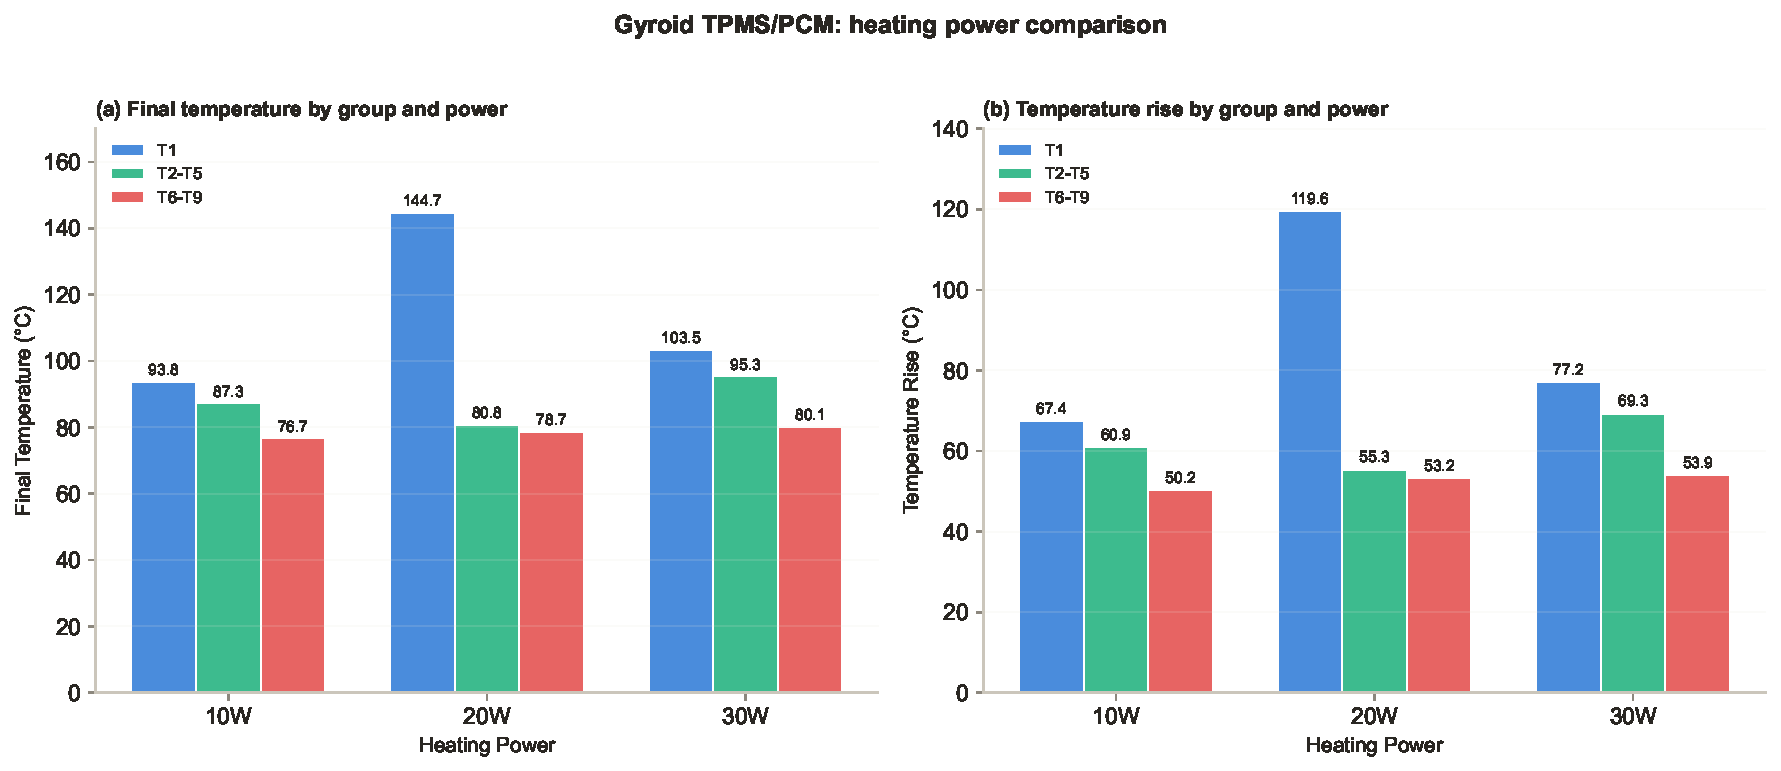
\includegraphics[width=\linewidth]{figures/fig_02_power_comparison.pdf}
\caption{(a)~Final temperatures and (b)~temperature rise by group and heating power for the Gyroid TPMS/PCM composite. Error in final temperature measurement: $\pm$0.1\textdegree C.}
\label{fig:comparison}
\end{figure}

\paragraph{Power-dependent behavior.}
Fig.~\ref{fig:comparison}b compares the temperature rise ($\Delta T = T_{\text{final}} - T_{\text{initial}}$) across power levels. For Group~A, the temperature rise increases from 67.5\textdegree C (10~W) to 119.5\textdegree C (20~W) to 77.2\textdegree C (30~W). The non-monotonic trend---with 20~W producing the highest temperature rise---reflects the interplay between heating power and experiment duration: at 20~W, the 11.1~min duration allows Group~A to accumulate substantial thermal energy, while at 30~W the shorter 8.5~min duration limits the total energy input despite the higher power.

For Groups B and C, the temperature rise shows a more monotonic trend from 10~W to 30~W, with the outer groups benefiting from the higher heating rates without reaching the extreme temperatures observed at Group~A. Specifically, Group~B rises from 60.9\textdegree C (10~W) to 69.3\textdegree C (30~W), and Group~C rises from 50.2\textdegree C (10~W) to 53.9\textdegree C (30~W).

Fig.~\ref{fig:duration} illustrates the inverse relationship between heating power and experiment duration, highlighting the efficiency trade-off: higher power reduces the time to reach thermal equilibrium but may create larger thermal gradients within the composite.

\begin{figure}[htbp]
\centering
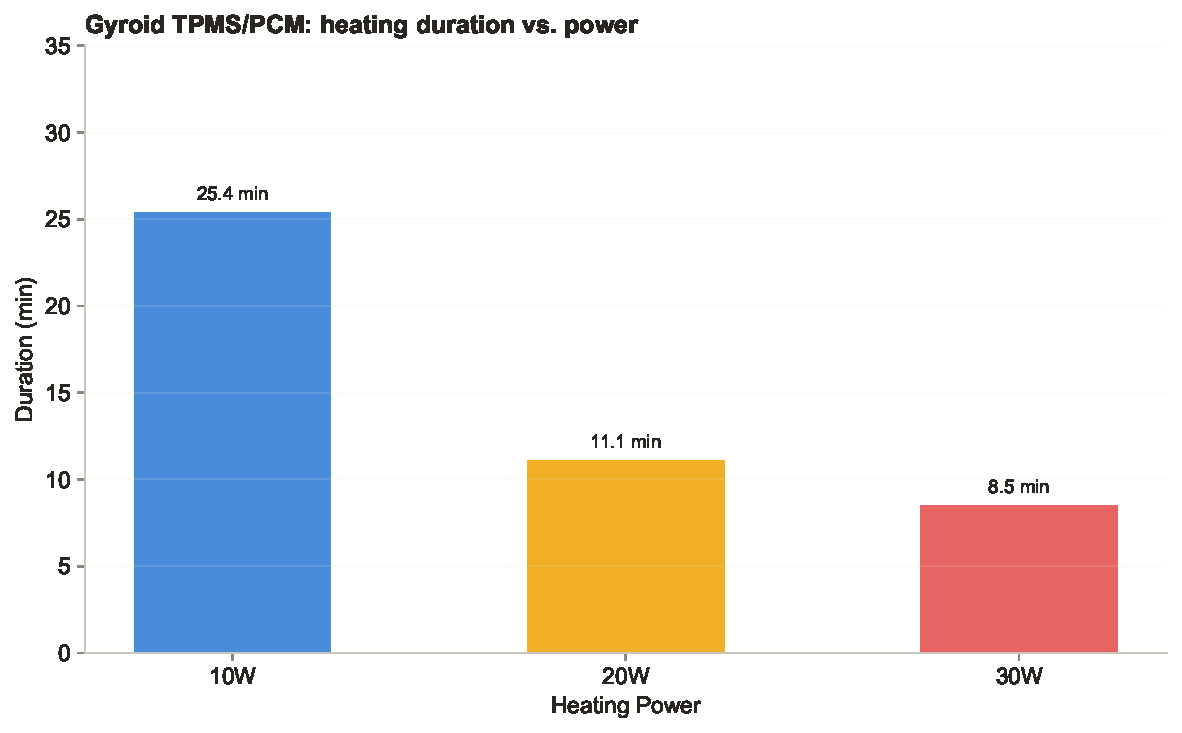
\includegraphics[width=0.7\linewidth]{figures/fig_03_duration.pdf}
\caption{Heating duration versus power for the Gyroid TPMS/PCM composite.}
\label{fig:duration}
\end{figure}

\paragraph{Outlier sensor analysis.}
The systematic identification of outlier sensors (Table~\ref{tab:outliers}) reveals spatially consistent patterns. $T_6$ was identified as an outlier in Group~C at both 10~W and 30~W, suggesting a position-dependent thermal anomaly---possibly due to imperfect thermal contact with the PCM or a slightly different local lattice geometry. The variation of the Group~B outlier ($T_3$ at 10/20~W vs.\ $T_5$ at 30~W) suggests that the thermal field within the intermediate region is sensitive to the heating rate, potentially reflecting different convection patterns in the molten PCM at different power levels~\cite{parida2020effect,cao2021characterization}.

\paragraph{Implications for TPMS-enhanced PCM.}
The results demonstrate that the AlSiMg Gyroid TPMS lattice provides effective thermal conductivity enhancement for the paraffin PCM. At 10~W, the temperature spread between the innermost and outermost sensor groups (17.1\textdegree C) is substantially smaller than what would be expected in a bare PCM system, where thermal gradients of 30--50\textdegree C are typical~\cite{souayfane2018melting}. The TPMS lattice acts as a distributed heat transfer network, conducting heat from the central heater radially outward through its high-conductivity metallic struts while the PCM absorbs and stores thermal energy through phase change.

The relatively small temperature difference between Groups B and C (10.6\textdegree C at 10~W, 2.1\textdegree C at 20~W, 15.2\textdegree C at 30~W) suggests that the TPMS lattice effectively homogenizes the temperature field in the outer region, which is advantageous for uniform thermal energy storage. The larger spread at 30~W may reflect the shorter experiment duration, which limits the time available for lateral heat conduction to establish thermal equilibrium.

\section{Conclusions}
\label{sec:conclusion}

This study presented an experimental investigation of paraffin-based PCM (phase change temperature 42\textdegree C) infiltrated into AlSiMg Gyroid TPMS lattice structures fabricated by laser powder bed fusion. The thermal response was systematically characterized under three heating power levels (10~W, 20~W, 30~W) using a nine-sensor array organized into three spatial groups. The key findings are:

\begin{enumerate}[nosep]
  \item The Gyroid TPMS lattice provides effective thermal conductivity enhancement, with the temperature spread between the innermost (Group~A) and outermost (Group~C) sensor groups limited to 17.1\textdegree C at 10~W---substantially smaller than typical bare PCM systems.

  \item A consistent radial thermal stratification ($T_1 > T_{2\text{-}5} > T_{6\text{-}9}$) was observed across all power levels, reflecting the heat flow direction from the central heater through the TPMS lattice/PCM composite.

  \item The heating power significantly affects the phase change dynamics: at 10~W, a clear phase change plateau near 42\textdegree C was observed for 5--8 minutes; at 20~W, the plateau compressed to 3--4 minutes; at 30~W, the plateau was barely discernible due to the high heating rate.

  \item The experiment duration decreased from 25.4~min (10~W) to 11.1~min (20~W) to 8.5~min (30~W), with the outer sensor groups (B and C) showing more monotonic temperature rise trends than the innermost group (A).

  \item Systematic outlier analysis revealed that $T_6$ was consistently identified as an outlier in Group~C, while the Group~B outlier varied with heating power, suggesting power-dependent convection patterns in the molten PCM.
\end{enumerate}

The present work establishes the Gyroid TPMS/PCM baseline for an ongoing comparative study. Future experiments will extend the test matrix to Primitive and IWP topologies at all three heating powers (Table~\ref{tab:test_matrix}), enabling direct comparison of the thermal performance across TPMS families. The comparative data will inform the selection of optimal TPMS topologies for specific thermal management applications, considering trade-offs between thermal response rate, temperature uniformity, and energy storage capacity.

Several limitations of the current study should be noted. First, only the heating (melting) phase has been characterized; the cooling (solidification) behavior of the TPMS/PCM composite remains to be investigated. Second, the current analysis is based solely on temperature measurements; future work should incorporate heat flux measurements and energy balance calculations to quantify the effective thermal conductivity enhancement factor. Third, the effect of natural convection within the molten PCM channels of the TPMS lattice has not been isolated; complementary numerical simulations using the enthalpy-porosity method~\cite{ebrahimi2019sensitivity} are planned to decompose the conduction and convection contributions.


% unsrtnat: number references by order of first citation (repeats reuse the number)
\bibliographystyle{unsrtnat}
\bibliography{bibliography}

\end{document}
